\chapter{RoboCup 3D Simulation League}
\label{Soccer Simulation League 3D}

The 3D Simulation League~\cite{SoccerSimulationLeague3D} increases the realism of the simulated environment used in the 2D Simulation League by adding an extra dimension and more complex physics. At its beginning, the only available robot model was a spherical agent. In 2006, a simple model of the Fujitsu HOAP-2 robot was made available, being the first time that humanoid models were used in the simulation league. This shifted the aim of the 3D Simulation League from the design of strategic behaviors in playing soccer towards some low-level control of humanoid robots and the creation of basic behaviors, like walking, kicking, turning and standing up, among others.

In 2008, the introduction of a Nao robot model to the simulation gave another perspective to the league. The real Nao robot from Aldebaran robotics has been the official robot for the Standard Platform League since 2008. Using the same model for the simulation competitions represents a great opportunity for researchers wanting to test their algorithms and ideas before trying them into the real robots. The interest in the 3D Simulation League is growing fast and research is slowly getting back to the design and implementation of multi-agent higher-level behaviors based on solid low-level behavior architectures for realistic humanoid robot teams. SimSpark is used as the official Robocup 3D simulator.

\section{SimSpark Soccer Simulator}
\textit{SimSpark}~\cite{SimSpark} is a generic physics simulator system for multiple agents in three-dimensional environments. It builds on the flexible Spark application framework. In comparison to specialized simulators, users can create new simulations by using a scene description language. SimSpark is a powerful tool to study different multi-agent research questions. 

\textit{Rcssserver3d} is the official competition environment for the RoboCup 3D Simulation League. It implements a simulated soccer environment, whereby two teams of up to nine, and in the latest version up to eleven, humanoid robots play against each other. Figure~\ref{fig:SimulationSoccerField} shows the dimensions and the layout of the simulated soccer field.

\begin{figure}[ht!]
\centering
  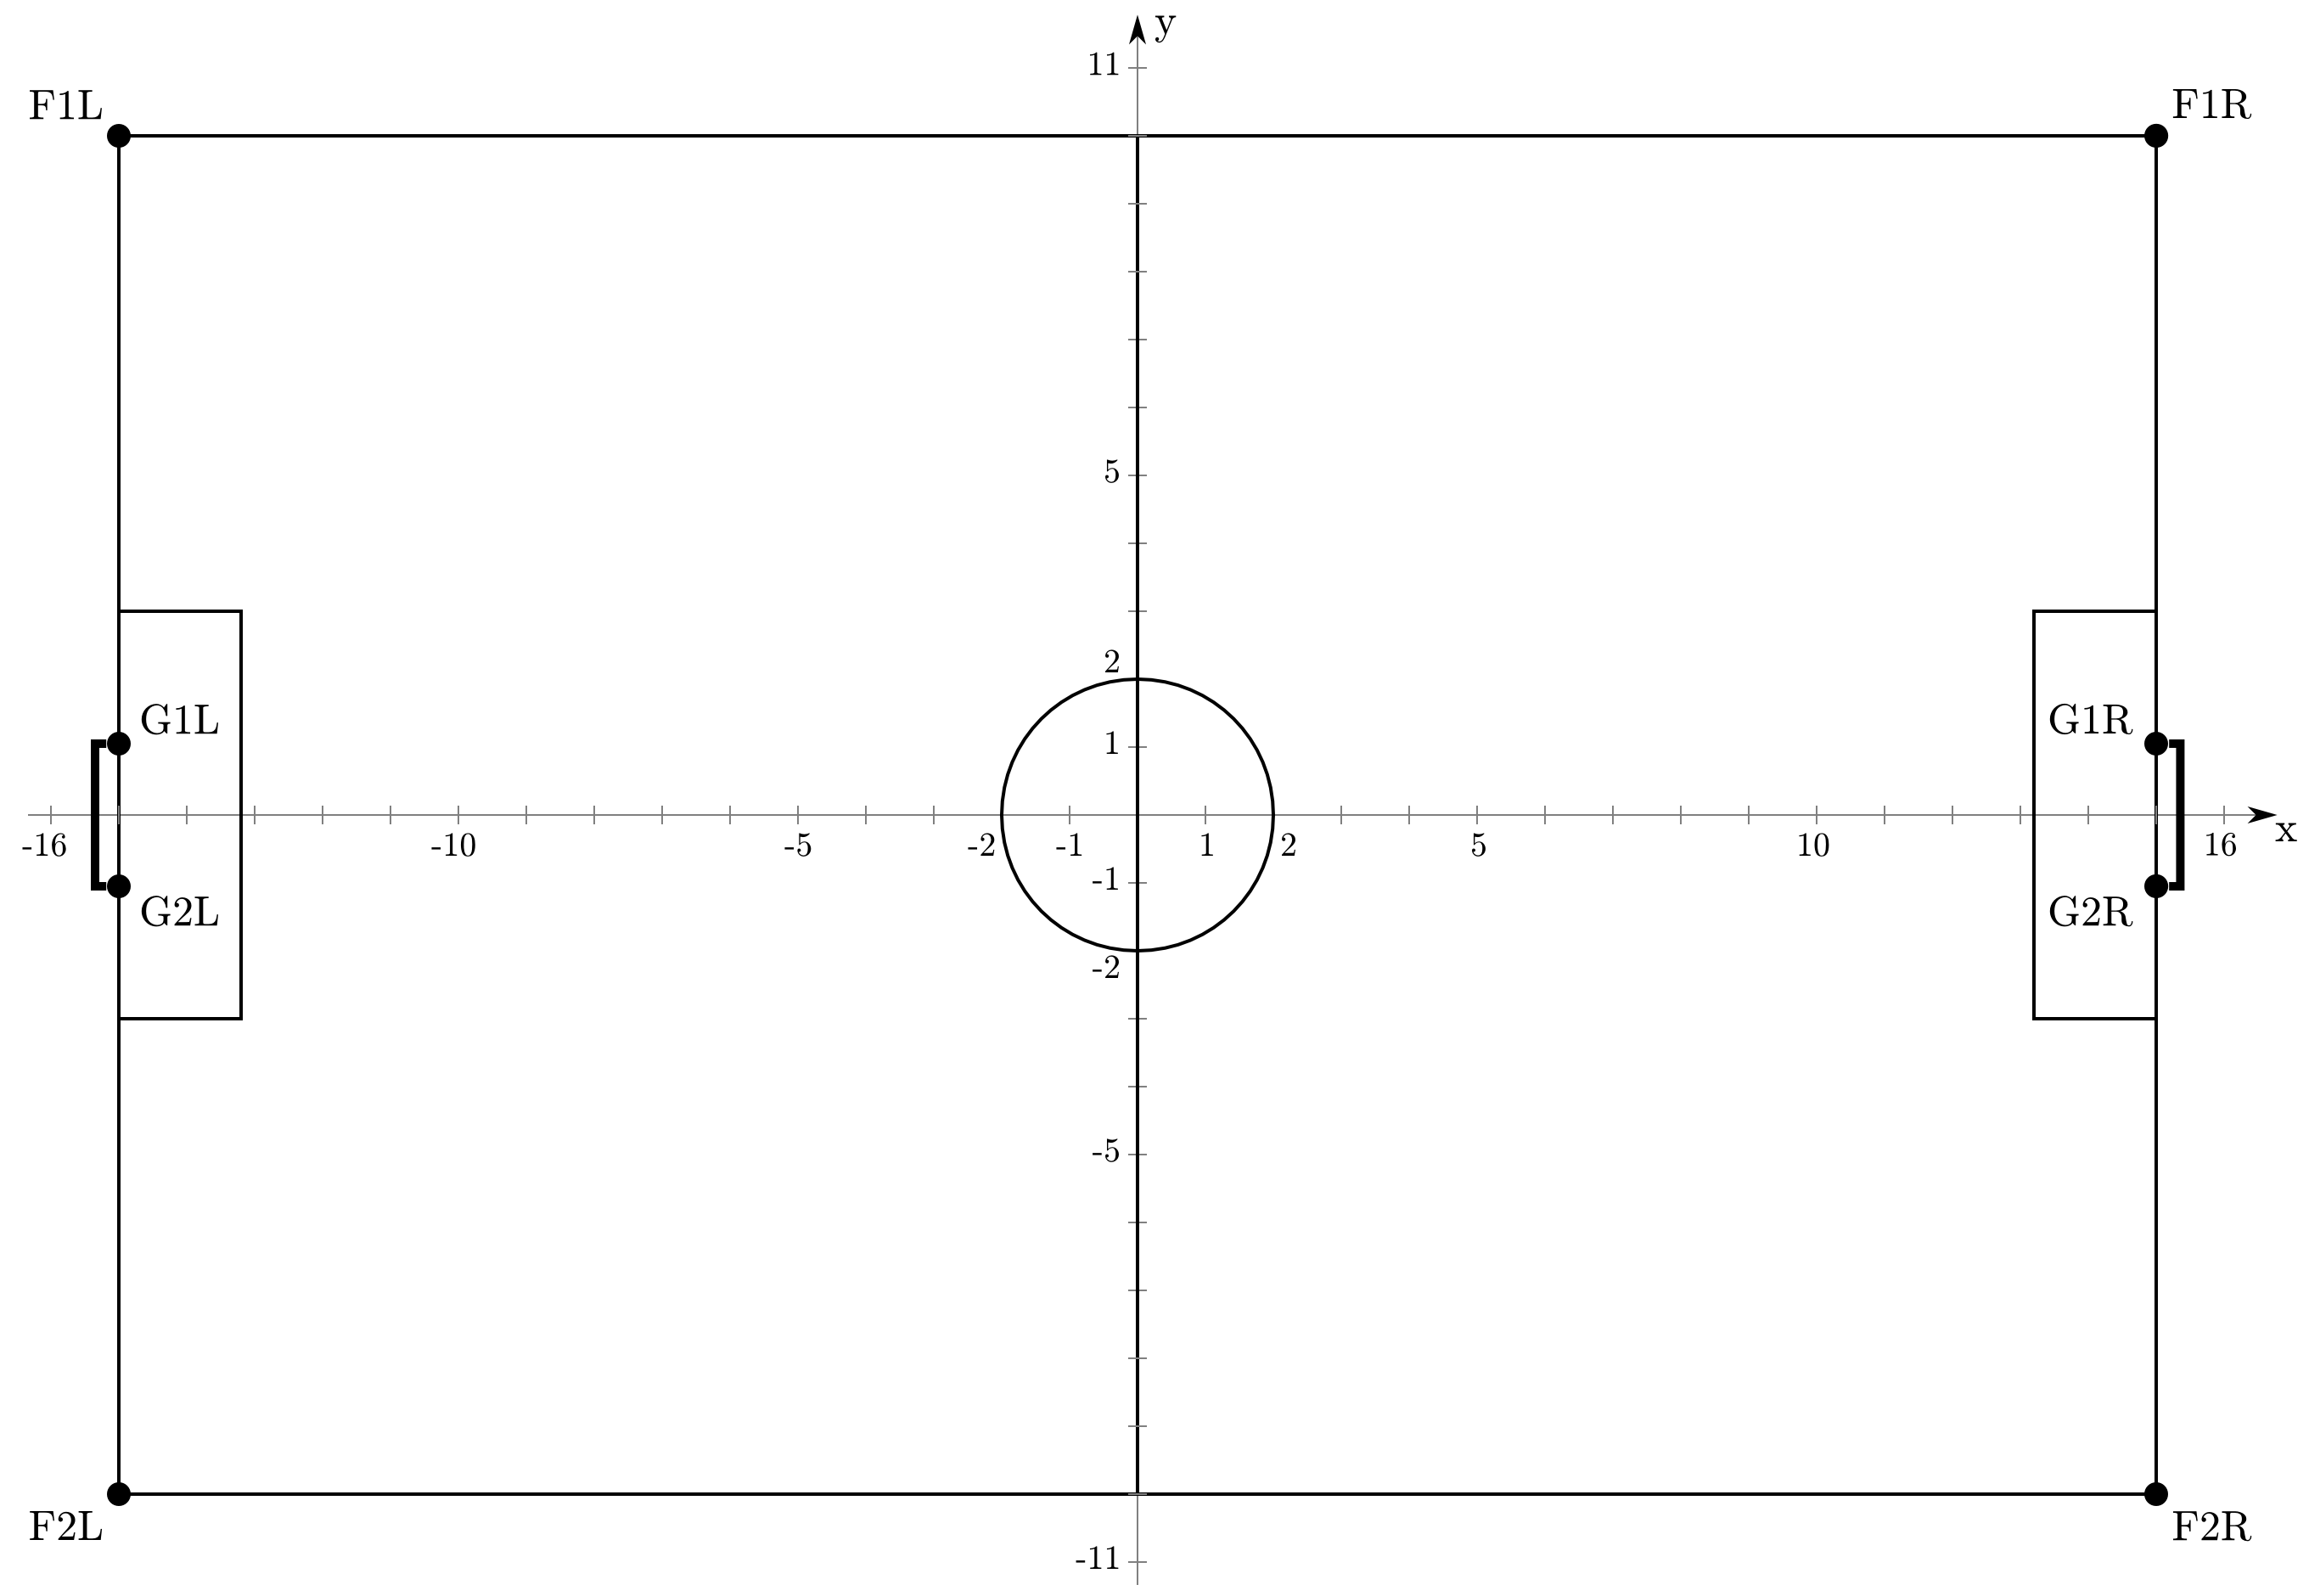
\includegraphics[width=0.8\textwidth]{Chapter2/figures/SoccerSimulation_FieldPlan.png}
  \caption{RoboCup 3D Simulation League Field} 
  \label{fig:SimulationSoccerField}
\end{figure}

\section{Server}
The SimSpark server hosts the process that manages and advances the simulation. The simulation state is constantly modified through the simulation update loop. Each simulation step corresponds to 20ms of simulated time. Objects in the scene change their state, i.e. one or more of their properties, such as position, speed, angular velocity, etc., due to inherent or external influences. These properties are under the control of a rigid body physical simulation that resolves collisions, applies drag, gravity, etc. Agents that take part in the simulation also modify objects with the help of their effectors, which may move and apply forces to other objects. SimSpark implements a simple internal event model that immediately executes every action received from an agent.


Another responsibility of the server is to keep track of connected agent processes. The SimSpark server exposes a network interface to all agents on TCP port 3100 (default value). In each simulation cycle, the server collects and reports sensor information for each of the sensors of all connected agents. It further carries out received action sequences triggered by the connected agents through their available effectors.
The server does not try to compensate for network latencies or differences in computing resources available to the connected agents. A consequence is that simulations are not reproducible. This means repeated simulations may have a different outcome, depending on network delays or load variations on the machines hosting the agents and the server.


\section{Monitor}

The server can render the simulation itself, depending on its configuration. It implements an internal monitor that omits the network overhead. However, it supports streaming data to remote monitor processes, which take responsibility for rendering the 3D scene for remote viewing.


\subsection{SimSpark Monitor}
The SimSpark monitor is responsible for rendering the current simulation. It connects to a running server instance from which it continuously receives a stream of updates that describe the simulation state, either as full snapshots or as incremental updates.
The format of the data stream the server sends to the monitor is called \textit{Monitor Format}. It is a customizable language used to describe the simulation state in text format.
Apart from describing the pure simulation state, each Monitor Format may provide a mechanism to transfer additional game-specific state. For the soccer simulation, this game-specific state may include, for example, current play mode and goals scored so far. The monitor client itself only renders the pure scene and defers the rendering of the game-specific state to plugins. These plugins are intended to parse the game-specific state and display it as an overlay printed out on screen.



\subsection{Roboviz Monitor}
\textit{RoboViz}~\cite{Roboviz} was created by Justin Stoecker in collaboration with the RoboCup group (RoboCanes) at the University of Miami's Department of Computer Science.
RoboViz is a software program designed to assess and debug agent behaviors in the RoboCup 3D Simulation League. RoboViz is an interactive monitor that renders agent and world state information in a three-dimensional scene. In addition, RoboViz provides programmable drawing and debug functionality to agents that can communicate over a network. The tool facilitates the real-time visualization of agents running concurrently on the SimSpark simulator and provides higher-level analysis and visualization of agent behaviors not currently possible with existing tools. Figure~\ref{fig:Roboviz} shows a visual comparison of the RoboViz and SimSpark Monitors.

\begin{figure}[!h] 
  \begin{center}
    \subfigure{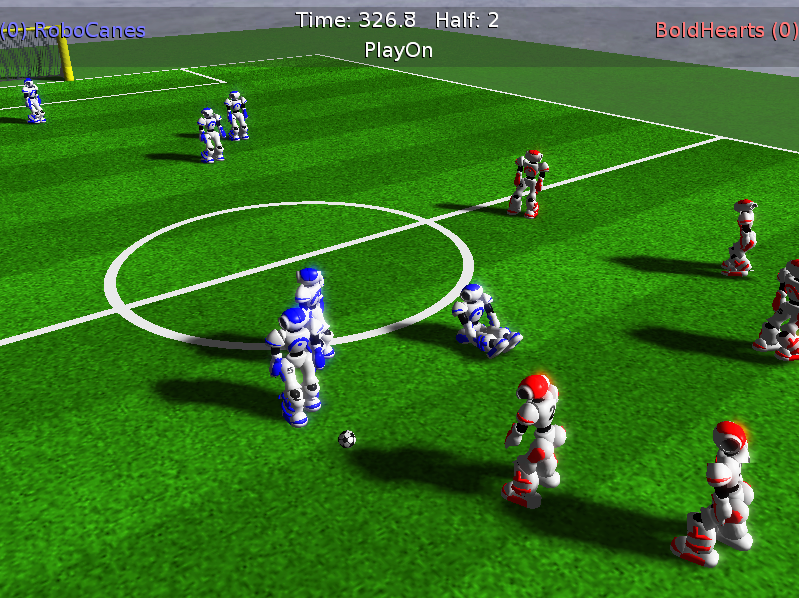
\includegraphics[width=0.4\textwidth]{Chapter2/figures/RobovizMonitor.png}}
    \subfigure{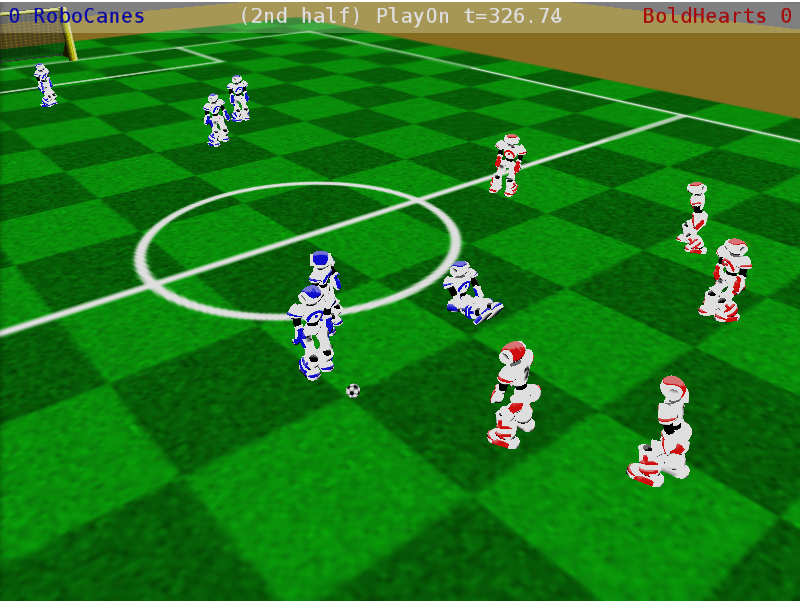
\includegraphics[width=0.4\textwidth]{Chapter2/figures/SimSparkMonitor.png}}
  \end{center}
  \caption{Roboviz (left) vs SimSpark (right) Monitors.}
  \label{fig:Roboviz}
\end{figure}





\section{Perceptors}
Perceptors are the senses of an agent, allowing awareness of the agent's model state and the environment.
The server sends perceptor messages to connected agents via the network protocol at each cycle of the simulation.
There are both general perceptors available in all simulations and soccer perceptors specific to the soccer simulation.



\subsection{General perceptors}

\begin{description}
  \item [HingeJoint Perceptor]
  A hinge joint perceptor receives information about the angle of the corresponding single-axis hinge joint. It contains the identifier \texttt{HJ}, the name of the perceptor, and the position angle of the axis in degrees. A zero angle corresponds to straightly aligned bodies. The position angle of each hinge joint perceptor is sent at each cycle.
Each hinge joint has minimum and maximum limits on its angular position. This varies from hinge to hinge and depends upon the model being used. Nao has 22 hinge joint perceptors, which are the only joint type used in this robot.

 \begin{description}
  \item[{\bf Message format:}]
  \texttt{(HJ (n <name>) (ax <ax>))}
  \item[{\bf Frequency:}]
  Every cycle
   \item[{\bf Noise Model:}] None, however values are truncated to two decimal places, equating to a uniform error of up to 0.01 degrees.
  \end{description}
  
  
  \item [ForceResistance Perceptor]
  This perceptor informs about the force that acts on a body.  After the identifier \texttt{FRP} and the name of the body, the perceptor message contains two three-dimensional vectors. The first vector describes the point of origin on the body where the force is applied to and the second vector is the force vector (magnitude and  direction) of the force applied to this point. This information is just an approximation of the real applied force. The point of origin is calculated as the weighted average of all contact points to which force is applied, while the force vector represents the total force applied to all of these contact points. The perceptor message for force resistance perceptors is sent only in case of a collision of the corresponding body with another simulated object. Nao has two of these perceptors, located in the bottom of each foot and labeled \texttt{lf} and \texttt{rf}.
 \begin{description}
  \item[{\bf Message format:}]
  \texttt{(FRP (n <name>) (c <px> <py><pz>) (f <fx><fy><fz>))}
  \item[{\bf Frequency:}]Only in cycles where a body collision occurs
  \item[{\bf Noise Model:}]
  None, however values are truncated to two decimal places, equating to a uniform error of up to 0.01 metres/newtons.
  \end{description}


  \item [GyroRate Perceptor]
  The gyro rate perceptor delivers information about the change in orientation of a body. The message contains the \texttt{GYR} identifier, the name of the body to which the gyro perceptor belongs to, and the rates of change of the three rotation (Euler) angles. These values describe the rates of change in orientation of the body during the last cycle, in other words the current angular velocities about the three rotation axes of the corresponding body in degrees per second. To keep track of the orientation of the body, the information to each gyro rate perceptor is sent at each cycle. Nao has a gyro perceptor in the upper torso.
  \begin{description}
  \item[{\bf Message format:}]
  \texttt{(GYR (n <name>) (rt <x> <y> <z>))}
  \item[{\bf Frequency:}]
  Every cycle
  \item[{\bf Noise Model:}]None, however values are truncated to two decimal places, equating to a uniform error of up to 0.01 degrees.
  \end{description}

  \item [Accelerometer Perceptor]
  This perceptor measures the proper acceleration a body experiences relative to free fall. As a consequence an accelerometer at rest relative to the simulated earth's surface will indicate an acceleration of approximately 1g upwards. To obtain the acceleration due to motion with respect to the earth, this gravity offset should be subtracted. After the identifier \texttt{ACC} and the name of the body, the perceptor message contains a three-dimensional vector with the acceleration values along the three Cartesian axes. Nao has an accelerometer in the upper torso.
    \begin{description}
  \item[{\bf Message format:}]
  \texttt{(ACC (n <name>) (a <x> <y> <z>))}
  \item[{\bf Frequency:}]
  Every cycle
  \item[{\bf Noise Model:}]None, however values are truncated to two decimal places, equating to a uniform error of up to 0.01 m/$s^{2}$.
  \end{description}
\end{description}

\subsection{Soccer perceptors}

\begin{description}
  \item [Vision Perceptor]
  Most important perceptor of the Nao robot is the vision perceptor which delivers information about seen objects in the environment, where objects are either others players, the ball, field-lines or markers on the field. Currently there are 8 markers on the field: one at each corner point of the field and one at each goal post. With each visible object you get a vector described in spherical coordinates. In other words the distance together with the horizontal and latitudal angle to the center of a visible object relative to the orientation of the camera. Nao possess a restricted vision perceptor at the center of it's head. This perceptor's type is \texttt{RestrictedVisionPerceptor} which limits the field of view to $120^{\circ}$. This limitation has major importance in the part of self-localization we are going to see in the next chapter.

 \begin{description}
  \item[{\bf Message format:}]
  \begin{verbatim}
  (See +(<name> (pol <distance> <angle1>
   <angle2>))+(P (team <teamname>) (id <playerID>)
   + (<bodypart> (pol <distance> <angle1> <angle2
   >)))+(L (pol <distance> <angle1> <angle2>)(pol
   <distance> <angle1> <angle2>)))
  \end{verbatim}
  \item[{\bf Frequency:}]
 Every third cycle (60ms)
  \item[{\bf Noise Model:}]Calibration error (a fixed offset of around $\pm$0.004m in each of x/y/z axes), Gaussian noise  and values are truncated to two decimal places, equating to a uniform error of up to 0.01.
  \end{description}


  \item [Hear Perceptor]
  Agent processes are not allowed to communicate with each other directly, but agents may exchange messages via the simulation server. For this purpose agents are equipped with the so-called hear perceptor, which serves as an aural sensor and receives messages shouted by other players. A hear perceptor message is started with the \texttt{hear} identifier, followed by the simulation time at which the given message was heard in seconds, either a relative horizontal direction in degrees indicating where the sound originated, or \texttt{self} indicating that the player is hearing their own shouted message, and finally the message itself.
  \begin{description}
  \item[{\bf Message format:}]
  \texttt{(hear <time> self/<direction> <message>)}
  \item[{\bf Frequency:}]
  Every cycle
  \end{description}

The hear perceptor comes up with some restrictions which we are going to present in the next chapter in communication's section.
  
  
    \item [GameState Perceptor]
  The game state perceptor delivers several information about the actual state of the soccer game environment. A game state message is started with the \texttt{GS} identifier, followed by a list of different state information. Currently just the actual play time and play mode are transmitted in each cycle. Play time starts from zero at kickoff of the first half, and 300 at kickoff of the second half and is given as a floating point number in seconds, to two decimal places.
     \begin{description}
  \item[{\bf Message format:}]
  \texttt{(GS (t <time>) (pm <playmode>))}
  \item[{\bf Frequency:}]
 Every cycle
  \end{description}
%These game states are: BeforeKickOff, PlayOn, KickOff_Left, KickOff_Right, Goal_Left, GoalRight, KickInLeft, KickInRight, corner_kick_left, corner_kick_right, goal_kick_left, goal_kick_right.

\end{description}
\section{Effectors}

Effectors allow agents to perform actions within the simulation. Agents control them by sending messages to the server, and the server changes the game state accordingly. Effectors are the logical dual of perceptors.
Effector control messages are sent via the network protocol. There are both general effectors that apply to all simulations, and soccer effectors that are specific to the soccer simulation.\\
\subsection{General Effectors}
\begin{description}


  \item [Create Effector]
  When an agent initially connects to the server it is invisible and cannot take affect a simulation in any meaningful way. It only possesses a so-called CreateEffector. An agent uses this effector to advice the server to construct it according to a scene description file it passes as a parameter. This file is used to construct the physical representation and all further effectors and perceptors.
  \begin{description}
  \item[{\bf Message format:}]
  \texttt{(scene <filename>)}
  \end{description}

  \item [HingeJoint Effector]
  Effector for all axis with a single degree of freedom. The first parameter is the name of the axis. The second parameter is a speed value, passed in radians per second. Setting a speed value on a hinge means that the speed will be maintained until a new value is provided. Even if the hinge meets its extremity, it will bounce around at the extremity until a new speed value is requested.
  \begin{description}
  \item[{\bf Message format:}]
  \texttt{(<name> <ax>)}
  \end{description}

  \item [Synchronize Effector]
  Agents running in Agent Sync Mode must send this command at the end of each simulation cycle. Note that the server ignores this command if it is received in Real-Time Mode, so it is safe to configure your agent to always append this command to your agent's responses.
  \begin{description}
  \item[{\bf Message format:}]
  \texttt{(syn)}
  \end{description}

\end{description}




\subsection{Soccer Effectors}


\begin{description}


  \item [Init Effector]
  The init command is sent once for each agent after the create effector sent the scene command. It registers this agent as a member of the passed team with the passed number. All players of one team have to use the same teamname and different player number values. When an agent connects to the server, he must first send a \texttt{CreateEffector} message followed by an \texttt{InitEffector} message in order to initialize himself into the soccer field.
  \begin{description}
  \item[{\bf Message format:}]  
  \texttt{(init (unum <playernumber>)\\(teamname <teamname>)) }
  \end{description}



  \item [Beam Effector]
  The beam effector allows a player to position itself on the field before the start of each half. The x and y coordinates define the position on the field with respect to the field's coordinate system, where (0,0) is the absolute center of the field. The rot specifies the facing angle of the player in degrees. Zero points to positive x-axis, 90 to positive y-axis.
  \begin{description}
  \item[{\bf Message format:}]  
  \texttt{(beam <x> <y> <rot>)}
  \end{description}



  \item [Say Effector]
  The say effector permits communication among agents by broadcasting messages. In order to say something, the following command has to be employed.
  \begin{description}
  \item[{\bf Message format:}]
  \texttt{(say <message>)}
  \end{description}

\end{description}
\section{Model}
SimSpark comes with Nao robot model for use by agents. The physical representation of each model is stored in an .rsg file.The Nao humanoid robot manufactured by Aldebaran Robotics. Its height is about 57cm and its weight is around 4.5kg. Its biped architecture with 22 degrees of freedom allows Nao to have great mobility. \textit{Rcssserver3d} simulates Nao nicely, Figure~\ref{fig:Naoinsimulationscreen} shows Nao's depiction into the Roboviz monitor.
\begin{figure}[ht]
\centering
  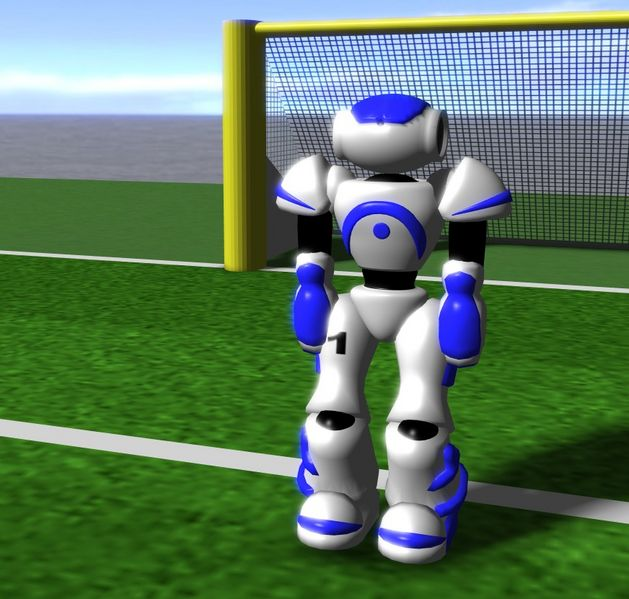
\includegraphics[scale=0.3]{Chapter2/figures/629px-Models-nao.jpg}
  \caption{Nao in Roboviz Monitor} 
  \label{fig:Naoinsimulationscreen}
\end{figure}